% --------------------------------------------------------------
% This is all preamble stuff that you don't have to worry about.
% Head down to where it says "Start here"
% --------------------------------------------------------------
 
\documentclass[12pt]{article}
\usepackage{amsgen,amsmath,amstext,amsbsy,amsopn,amssymb,mathabx,amsthm,bm,bbm,romannum,enumitem}
\usepackage[dvips]{graphicx}

\usepackage[pagebackref,bookmarksnumbered]{hyperref}
\usepackage{url}
\hypersetup{
	colorlinks=true,
	linkcolor=red,
	filecolor=magenta,      
	urlcolor=blue,
}

\setcounter{tocdepth}{3}
\usepackage[depth=3]{bookmark}

\usepackage[margin=1in]{geometry}
\renewcommand{\baselinestretch}{1.5}	% Line Stretch

\usepackage[utf8]{inputenc}

%----- theorems -----%

\newtheorem{thm}{Theorem}[section]
\newtheorem{lem}[thm]{Lemma}
\newtheorem{prop}[thm]{Proposition}
\newtheorem{coro}[thm]{Corollary}

\theoremstyle{definition}
\newtheorem{dfn}{Definition}[section]
\newtheorem*{pchln}{Punchline}

\theoremstyle{remark}
\newtheorem*{rmk}{Remark}
\newtheorem*{note}{Note}
\newtheorem{eg}{Example}[section]
\newtheorem{fact}{Fact}[section]
\newtheorem*{hint}{Hint}


%----- bold fonts -----%

\newcommand{\ab}{\mathbf{a}}
\newcommand{\bbb}{\mathbf{b}}
\newcommand{\cbb}{\mathbf{c}}
\newcommand{\db}{\mathbf{d}}
\newcommand{\eb}{\mathbf{e}}
\newcommand{\fb}{\mathbf{f}}
\newcommand{\gb}{\mathbf{g}}
\newcommand{\hb}{\mathbf{h}}
\newcommand{\ib}{\mathbf{i}}
\newcommand{\jb}{\mathbf{j}}
\newcommand{\kb}{\mathbf{k}}
\newcommand{\lb}{\mathbf{l}}
\newcommand{\mb}{\mathbf{m}}
\newcommand{\nbb}{\mathbf{n}}
\newcommand{\ob}{\mathbf{o}}
\newcommand{\pb}{\mathbf{p}}
\newcommand{\qb}{\mathbf{q}}
\newcommand{\rb}{\mathbf{r}}
\newcommand{\sbb}{\mathbf{s}}
\newcommand{\tb}{\mathbf{t}}
\newcommand{\ub}{\mathbf{u}}
\newcommand{\vb}{\mathbf{v}}
\newcommand{\wb}{\mathbf{w}}
\newcommand{\xb}{\mathbf{x}}
\newcommand{\yb}{\mathbf{y}}
\newcommand{\zb}{\mathbf{z}}

% denote vectors
\newcommand{\ba}{\bm{a}}
\newcommand{\bb}{\bm{b}}
\newcommand{\bc}{\bm{c}}
\newcommand{\bd}{\bm{d}}
\newcommand{\be}{\bm{e}}
\newcommand{\bbf}{\bm{f}}
\newcommand{\bg}{\bm{g}}
\newcommand{\bh}{\bm{h}}
\newcommand{\bi}{\bmf{i}}
\newcommand{\bj}{\bm{j}}
\newcommand{\bk}{\bm{k}}
\newcommand{\bl}{\bm{l}}
\newcommand{\bbm}{\bm{m}}
\newcommand{\bn}{\bm{n}}
\newcommand{\bo}{\bm{o}}
\newcommand{\bp}{\bm{p}}
\newcommand{\bq}{\bm{q}}
\newcommand{\br}{\bm{r}}
\newcommand{\bs}{\bm{s}}
\newcommand{\bt}{\bm{t}}
\newcommand{\bu}{\bm{u}}
\newcommand{\bv}{\bm{v}}
\newcommand{\bw}{\bm{w}}
\newcommand{\bx}{\bm{x}}
\newcommand{\by}{\bm{y}}
\newcommand{\bz}{\bm{z}}

% denote random matrices
\newcommand{\Ab}{\mathbf{A}}
\newcommand{\Bb}{\mathbf{B}}
\newcommand{\Cb}{\mathbf{C}}
\newcommand{\Db}{\mathbf{D}}
\newcommand{\Eb}{\mathbf{E}}
\newcommand{\Fb}{\mathbf{F}}
\newcommand{\Gb}{\mathbf{G}}
\newcommand{\Hb}{\mathbf{H}}
\newcommand{\Ib}{\mathbf{I}}
\newcommand{\Jb}{\mathbf{J}}
\newcommand{\Kb}{\mathbf{K}}
\newcommand{\Lb}{\mathbf{L}}
\newcommand{\Mb}{\mathbf{M}}
\newcommand{\Nb}{\mathbf{N}}
\newcommand{\Ob}{\mathbf{O}}
\newcommand{\Pb}{\mathbf{P}}
\newcommand{\Qb}{\mathbf{Q}}
\newcommand{\Rb}{\mathbf{R}}
\newcommand{\Sbb}{\mathbf{S}}
\newcommand{\Tb}{\mathbf{T}}
\newcommand{\Ub}{\mathbf{U}}
\newcommand{\Vb}{\mathbf{V}}
\newcommand{\Wb}{\mathbf{W}}
\newcommand{\Xb}{\mathbf{X}}
\newcommand{\Yb}{\mathbf{Y}}
\newcommand{\Zb}{\mathbf{Z}}

% denote random vectors
\newcommand{\bA}{\bm{A}}
\newcommand{\bB}{\bm{B}}
\newcommand{\bC}{\bm{C}}
\newcommand{\bD}{\bm{D}}
\newcommand{\bE}{\bm{E}}
\newcommand{\bF}{\bm{F}}
\newcommand{\bG}{\bm{G}}
\newcommand{\bH}{\bm{H}}
\newcommand{\bI}{\bm{I}}
\newcommand{\bJ}{\bm{J}}
\newcommand{\bK}{\bm{K}}
\newcommand{\bL}{\bm{L}}
\newcommand{\bM}{\bm{M}}
\newcommand{\bN}{\bm{N}}
\newcommand{\bO}{\bm{O}}
\newcommand{\bP}{\bm{P}}
\newcommand{\bQ}{\bm{Q}}
\newcommand{\bR}{\bm{R}}
\newcommand{\bS}{\bm{S}}
\newcommand{\bT}{\bm{T}}
\newcommand{\bU}{\bm{U}}
\newcommand{\bV}{\bm{V}}
\newcommand{\bW}{\bm{W}}
\newcommand{\bX}{\bm{X}}
\newcommand{\bY}{\bm{Y}}
\newcommand{\bZ}{\bm{Z}}

% denote vectors
\newcommand{\bbeta}{\bm{\beta}}
\newcommand{\balpha}{\bm{\alpha}}
\newcommand{\bgamma}{\bm{\gamma}}
\newcommand{\blambda}{\bm{\lambda}}
\newcommand{\bomega}{\bm{\omega}}
\newcommand{\bmu}{\bm{\mu}}
\newcommand{\bepsilon}{\bm{\epsilon}}
\newcommand{\btheta}{\bm{\theta}}
\newcommand{\bphi}{\bm{\phi}}
\newcommand{\bvarphi}{\bm{\varphi}}
\newcommand{\bxi}{\bm{\xi}}
\newcommand{\bpi}{\bm{\pi}}

% denote matrices
\newcommand{\bGamma}{\bm{\Gamma}}
\newcommand{\bLambda}{\bm{\Lambda}}
\newcommand{\bSigma}{\bm{\Sigma}}

% others
\newcommand{\bcE}{\bm{\mathcal{E}}}	% filtration
\newcommand{\bcF}{\bm{\mathcal{F}}}	% filtration
\newcommand{\bcG}{\bm{\mathcal{G}}}	% filtration


%----- double fonts -----%

\newcommand{\bbR}{\mathbb{R}}
\newcommand{\bbE}{\mathbb{E}}
\newcommand{\bbN}{\mathbb{N}}
\newcommand{\bbP}{\mathbb{P}}
\newcommand{\bbQ}{\mathbb{Q}}
\newcommand{\bbZ}{\mathbb{Z}}


%----- script fonts -----%

\newcommand{\cA}{\mathcal{A}}
\newcommand{\cB}{\mathcal{B}}
\newcommand{\cC}{\mathcal{C}}
\newcommand{\cD}{\mathcal{D}}
\newcommand{\cE}{\mathcal{E}}
\newcommand{\cF}{\mathcal{F}}
\newcommand{\cG}{\mathcal{G}}
\newcommand{\cH}{\mathcal{H}}
\newcommand{\cI}{\mathcal{I}}
\newcommand{\cJ}{\mathcal{J}}
\newcommand{\cK}{\mathcal{K}}
\newcommand{\cL}{\mathcal{L}}
\newcommand{\cM}{\mathcal{M}}
\newcommand{\cN}{\mathcal{N}}
\newcommand{\cO}{\mathcal{O}}
\newcommand{\cP}{\mathcal{P}}
\newcommand{\cQ}{\mathcal{Q}}
\newcommand{\cR}{\mathcal{R}}
\newcommand{\cS}{\mathcal{S}}
\newcommand{\cT}{\mathcal{T}}
\newcommand{\cU}{\mathcal{U}}
\newcommand{\cV}{\mathcal{V}}
\newcommand{\cW}{\mathcal{W}}
\newcommand{\cX}{\mathcal{X}}
\newcommand{\cY}{\mathcal{Y}}
\newcommand{\cZ}{\mathcal{Z}}


%----- special operators -----%

\newcommand{\argmin}{\mathop{\mathrm{argmin}}}
\newcommand{\argmax}{\mathop{\mathrm{argmax}}}

\newcommand{\bvar}{\textbf{Var}}
\newcommand{\bbias}{\textbf{Bias}}
\newcommand{\bcov}{\textbf{Cov}}
\newcommand{\bcor}{\textbf{Cor}}
\newcommand{\brank}{\textbf{rank}}
\newcommand{\bsign}{\textbf{sign}}
\newcommand{\bdiag}{\textbf{diag}}	% diagonal
\newcommand{\bdim}{\textbf{dim}}	% dimension
\newcommand{\btr}{\textbf{tr}}	    % trace
\newcommand{\bspan}{\textbf{span}}	% linear span
\newcommand{\bsupp}{\textbf{supp}}	% support
\newcommand{\bepi}{\textbf{epi}}	% epigraph

\newcommand{\perm}{\textbf{Perm}}	% permutation

\newcommand{\wass}{\textbf{Wass}}	% Wasserstein Distance
\newcommand{\ks}{\textbf{KS}}		% Kolomogov-Smirnov Distance

\newcommand{\brem}{\textbf{Rem}}		% remainders


\newcommand{\bzero}{{\mathbf{0}}}	% zero vector
\newcommand{\bone}{{\mathbf{1}}}	% all-one vector
\newcommand{\bbone}{{\mathbbm{1}}}	% indicator

\newcommand{\rmd}{\mathrm{d}}		% differentiation

\newcommand\indep{\protect\mathpalette{\protect\independenT}{\perp}}
\def\independenT#1#2{\mathrel{\rlap{$#1#2$}\mkern2mu{#1#2}}}	% independence

%----- distribution name -----%

\newcommand{\Exp}{\textbf{Exp}}
\newcommand{\Pois}{\textbf{Pois}}
\newcommand{\Gumb}{\textbf{Gumbel}}
\newcommand{\Bern}{\textbf{Bernoulli}}
\newcommand{\Bin}{\textbf{Bin}}
\newcommand{\NBin}{\textbf{NBin}}
\newcommand{\Multi}{\textbf{Multi}}
\newcommand{\Geo}{\textbf{Geo}}
\newcommand{\Hyper}{\textbf{Hyper}}
\newcommand{\SBM}{\textbf{SBM}}
\newcommand{\PoisProc}{\textbf{PoisProc}}

\usepackage{titling}

% Create subtitle command for use in maketitle
\newcommand{\subtitle}[1]{
	\posttitle{
		\begin{center}\large#1\end{center}
	}
}
 
\usepackage[margin=1in]{geometry} 
\usepackage{amsmath,amsthm,amssymb}
\usepackage{graphicx}
\usepackage{float}

\newcommand{\N}{\mathbb{N}}
\newcommand{\Z}{\mathbb{Z}}
 
\newenvironment{theorem}[2][Theorem]{\begin{trivlist}
\item[\hskip \labelsep {\bfseries #1}\hskip \labelsep {\bfseries #2.}]}{\end{trivlist}}
\newenvironment{lemma}[2][Lemma]{\begin{trivlist}
\item[\hskip \labelsep {\bfseries #1}\hskip \labelsep {\bfseries #2.}]}{\end{trivlist}}
\newenvironment{exercise}[2][Exercise]{\begin{trivlist}
\item[\hskip \labelsep {\bfseries #1}\hskip \labelsep {\bfseries #2.}]}{\end{trivlist}}
\newenvironment{reflection}[2][Reflection]{\begin{trivlist}
\item[\hskip \labelsep {\bfseries #1}\hskip \labelsep {\bfseries #2.}]}{\end{trivlist}}
\newenvironment{proposition}[2][Proposition]{\begin{trivlist}
\item[\hskip \labelsep {\bfseries #1}\hskip \labelsep {\bfseries #2.}]}{\end{trivlist}}
\newenvironment{corollary}[2][Corollary]{\begin{trivlist}
\item[\hskip \labelsep {\bfseries #1}\hskip \labelsep {\bfseries #2.}]}{\end{trivlist}}

\def\name{Zhenghan Fang}

\usepackage{fancyhdr}
\pagestyle{fancy}
\fancyhf{}
\rhead{\name}
\cfoot{\thepage}
\renewcommand{\headrulewidth}{0pt}

\begin{document}

% --------------------------------------------------------------
%                         Start here
% --------------------------------------------------------------
 
%\renewcommand{\qedsymbol}{\filledbox}

\pagenumbering{arabic}

\title{STOR 614 - Linear Programming, Spring 2019 \\
Homework No. 3}
\author{\name}

\maketitle

\noindent
\textbf{Problem 1.}

\begin{proof}
~
\begin{enumerate}
\item If.

If a basis of $x^*$ and a basis of $y^*$ share $m-1$ elements, then the two bases also share $n-m-1$ nonbasic variables. Let $\{N(1),  ,N(n-m-1)\}$ be the indices of the shared nonbasic variables. Then $x^*$ and $y^*$ share the following $n-1$ linearly independent active constraints
\begin{align*}
    \begin{cases}
    Ax=b \\
    x_{N(1)} = 0 \\
    \vdots \\
    x_{N(n-m-1)} = 0
    \end{cases}
\end{align*}
Therefore, $x^*$ and $y^*$ are adjacent.

\item Only if.
\begin{lemma}{1}
Let $X$ be a set of vectors. If there are $n$ linearly independent vectors in $X$, and $x_i, \hdots, x_m \in X$ are linearly independent, then there exists a set of $n$ linearly independent vectors in $X$ that contains $x_i, \hdots, x_m$.
\end{lemma}

Let $S$ be the set of active constraints shared by $x^*$ and $y^*$. Let $T$ be the set of $m$ linealy independent constraints imposed by $Ax=b$. Then, $T \subseteq S$ and $S$ contains $n-1$ linearly independent elements. By Lemma 1, there exists $P \subseteq S$, such that $P$ has $n-1$ elements, the elements of $P$ are linearly independent, and $T \subseteq P$. Moreover, there exists a set of $n$ linearly independent active constraints for $x^*$, $B_x$, and a set of $n$ linearly independent active constraints for $y^*$, $B_y$, such that $P \subseteq B_x$, $P \subseteq B_y$. Then the bases corresponding to $B_x$ and $B_y$ share $m-1$ elements.
\end{enumerate}
\end{proof}

\vspace{\baselineskip}
\noindent
\textbf{Problem 2.}

\noindent
\textbf{(a)} 
\begin{proof}
If the reduced cost of every nonbasic variable is positive, then the object function reaches its maximum if and only if all nonbasic variables are zero. $x^*$ is the only solution that satisfies that all nonbasic variables are zero. Therefore, $x^*$ is the unique optimal solution.
\end{proof}

\noindent
\textbf{(b)}
\begin{proof}
Let $ x_B = \begin{bmatrix} x_{B(1)} \\ \vdots \\ x_{B(m)} \end{bmatrix} $ be the vector of basic variables in $x^*$, and $ x_N = \begin{bmatrix} x_{N(1)} \\ \vdots \\ x_{N(n-m)} \end{bmatrix} $ be the vector of nonbasic variables in $x^*$.
The constraints of the linear programming problem can be written as
\[
\begin{bmatrix} \Ib_{m} & \Pb \end{bmatrix} \begin{bmatrix} x_B \\ x_N \end{bmatrix} = b
\]
where $\Ib_{m} \in \bbR^{m\times m}$ is identity matrix, $\Pb \in \bbR^{m\times (n-m)}$, and $b \in \bbR^{m}$.

Suppose that $x_{N(k)}$ has a nonpositive reduced cost, $c$. Because $x^*$ is nondegenerate, all $b_i > 0$. Then there exists a feasible solution $x^{**}$ which satisfies
\[
\begin{cases}
x^{**}_{N(k)} > 0 \\
x^{**}_{N(i)} = 0 & i \ne k
\end{cases}
\]
The objective function $z(x^{**}) = K - cx^{**}_{N(k)} \ge K - cx^{*}_{N(k)} = z(x^{*})$, where $x^{*}_{N(k)} = 0$ and $K$ is a constant. This contradicts with that $x^*$ is the unique optimal solution.
\end{proof}

\noindent
\textbf{Problem 3.}

\noindent
\textbf{(a)}
Standard form.
\begin{alignat*}{9}
    &\text{max} \quad && z = \quad && 2x_1 + x_2         &&       \\
    &\text{s.t}       &&           && x_1 - x_2 + s_1    && = 2, \\
    &                 &&           && x_1 + x_2 + s_2    && = 6, \\
    &                 &&           && x_1, x_2, s_1, s_2 &&\ge 0
\end{alignat*}

Simplex method. Boxed number indicate the pivot element.
\begin{equation*}
  \begin{array}{ccccc|c|c|c}
    z &  x_1      &  x_2 &  s_1 &  s_2 &   \text{rhs} & \text{Basic var} & \text{Ratio test} \\ \hline
    1 &   -2      &   -1 &    0 &    0 &     0        &  z=0             &                   \\
    0 & \boxed{1} &   -1 &    1 &    0 &     2        &  s_1 = 2         & 2/1=2             \\
    0 &    1      &    1 &    0 &    1 &     6        &  s_2 = 6         & 6/1=6             \\ \hline\hline
    
    1 &    0 &        -3 &    2 &    0 &     4        &  z=4             &                   \\
    0 &    1 &        -1 &    1 &    0 &     2        &  x_1 = 2         & \text{N/A}        \\
    0 &    0 & \boxed{2} &   -1 &    1 &     4        &  s_2 = 4         & 4/2=2             \\ \hline\hline
    
    1 &    0 &         0 &  1/2 &          3/2 &    10        &  z=10            &                   \\
    0 &    1 &         0 &  1/2 &          1/2 &     4        &  x_1 = 4         &          \\
    0 &    0 &         1 & -1/2 &          1/2 &     2        &  x_2 = 2         &          \\ \hline\hline
  \end{array}
\end{equation*}
The BFS \[ (x_1,x_2,s_1,s_2) = (4,2,0,0) \] is optimal, and the optimal objective function value is $z=10$.

\noindent
\textbf{(b)}

\begin{figure}[H]
    \centering
    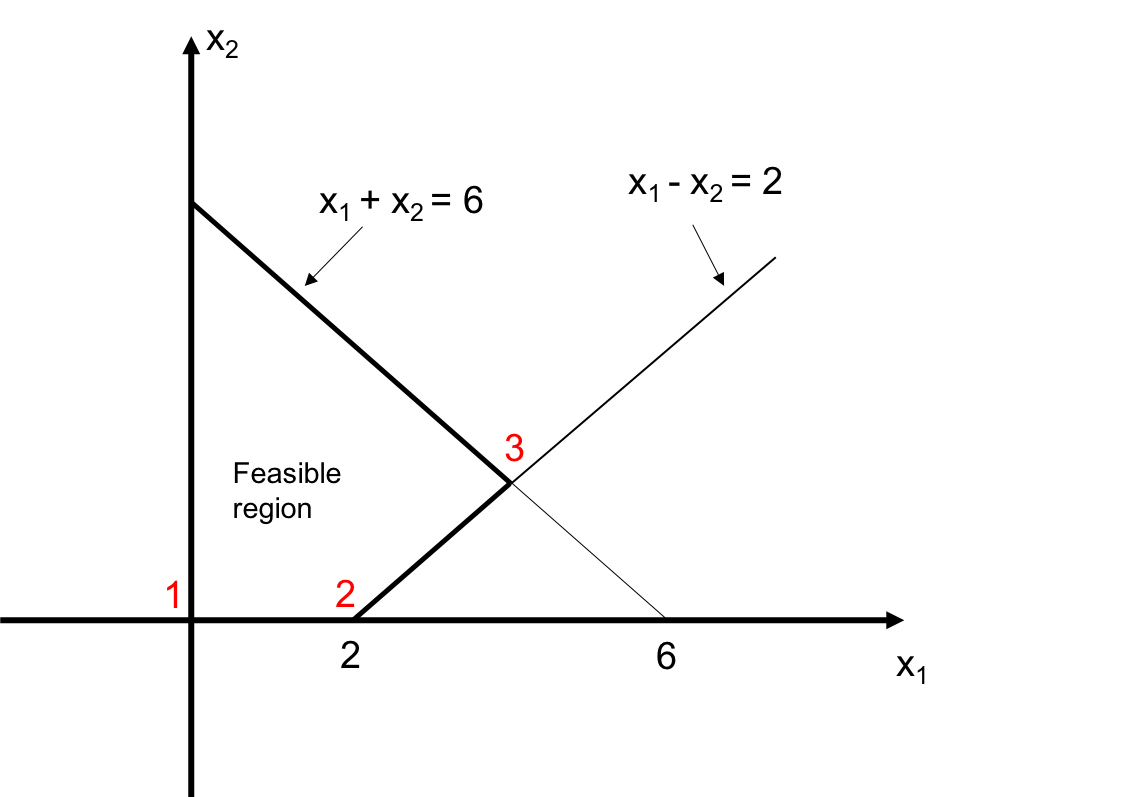
\includegraphics[width=4.5in]{Picture1.png}
    \caption{Optimization path of simplex method. Red numbers indicate the order of the BFS's reached in the simplex method.}
    \label{fig:my_label}
\end{figure}

\noindent
\textbf{Problem 4.}

\noindent
\textbf{(a)}
False.
\begin{proof}
If the feasible solution is moved by a positive distance, then the right-hand-side of the pivot row is positive, then the z-value must be changed (increased).
\end{proof}

\noindent
\textbf{(b)}
True.
\begin{proof}
Let $c$ be the reduced cost of the entering variable, $p$ be the pivot element, and $x^*$ be the leaving variable in one iteration. If the rules of simplex method are strictly followed, then $c<0$, $p>0$. Let $d$ be the new reduced cost of $x^*$ after that iteration, then $d = -c/p > 0 $. Therefore, the new reduced cost of the leaving variable must be positive. Therefore, the leaving variable cannot reenter in the very next iteration.
\end{proof}

\noindent
\textbf{(c)}
False. Counter example:
\begin{equation*}
  \begin{array}{ccccc|c|c|c}
    z &  x_1      &  x_2 &  s_1 &  s_2 &   \text{rhs} & \text{Basic var} & \text{Ratio test} \\ \hline
    1 &   -2      &   -8 &    0 &    0 &     0        &  z=0             &                   \\
    0 & \boxed{1} &    2 &    1 &    0 &     2        &  s_1 = 2         & 2/1=2             \\
    0 &    0      &    1 &    0 &    1 &     6        &  s_2 = 6         & \text{N/A}        \\ \hline\hline
    
    1 &    0 &        -4 &    2 &    0 &     4        &  z=4             &                   \\
    0 &    1 & \boxed{2} &    1 &    0 &     2        &  x_1 = 2         & 2/2=1             \\
    0 &    0 &         1 &    0 &    1 &     6        &  s_2 = 6         & 6/1=6             \\ \hline\hline
  \end{array}
\end{equation*}
Boxed number indicates pivot element. $x_1$ just entered in the first iteration but leaves in the next iteration.

\noindent
\textbf{(d)}
False. Counter example:
\begin{equation*}
  \begin{array}{ccccc|c|c|c}
    z &  x_1      &  x_2 &  s_1 &  s_2 &   \text{rhs} & \text{Basic var} & \text{Ratio test} \\ \hline
    1 &    2      &    0 &    0 &    0 &     4        &  z=4             &                   \\
    0 &    1      &    2 &    1 &    0 &     2        &  s_1 = 2         &             \\
    0 &    1      &    1 &    0 &    1 &     6        &  s_2 = 6         &         \\ \hline
  \end{array}
\end{equation*}
This tableau shows a nondegenerate optimal solution 
\begin{gather*}
    (x_1,x_2,s_1,s_2) = (0,0,2,6), 
\end{gather*}
but there exists another optimal solution
\begin{gather*}
    (x_1,x_2,s_1,s_2) = (0,1,0,5).
\end{gather*}


% --------------------------------------------------------------
%     You don't have to mess with anything below this line.
% --------------------------------------------------------------

\end{document}